\section{Durchführung}
\label{sec:Durchführung}

\subsection{Versuchsaufbau}

Der Versuch ist \autoref{fig:abb5} entsprechend aufgebaut.

\begin{figure}[H]
    \centering
    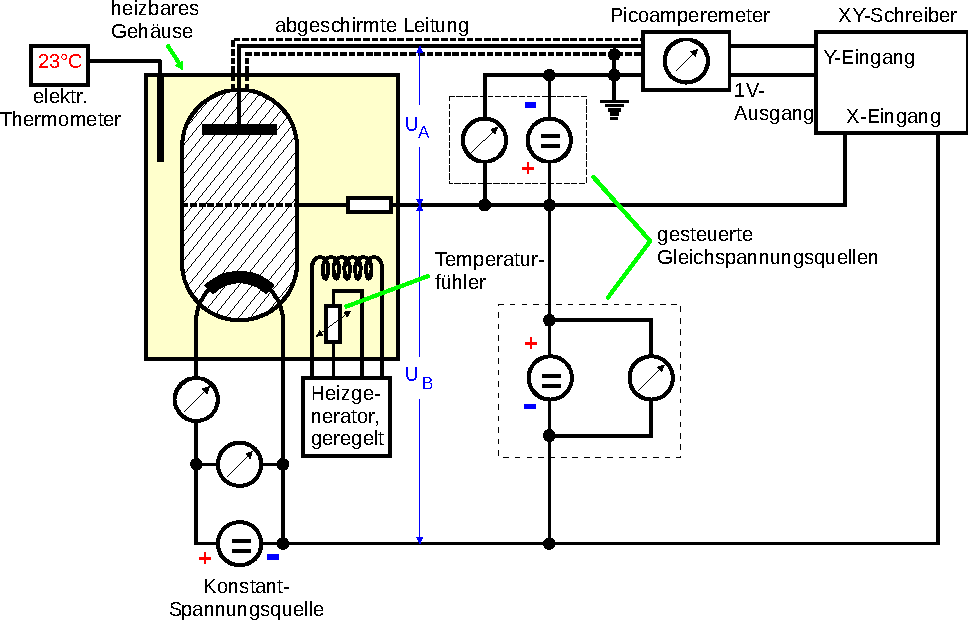
\includegraphics{figures/Abb_6.pdf}
    \caption{Schematische Darstellung des Versuchsaufbaus \cite{ap08}.}
    \label{fig:abb5}
\end{figure}

Im Wesentlichen besteht er aus einer Franck-Hertz-Röhre, an die eine Beschleunigungsspannung $0 \,\unit{\volt} \leq U_\text{B} \leq 60 \,\unit{\volt}$ 
und eine Bremsspannung $0 \,\unit{\volt} \leq U_\text{A} \leq 10 \,\unit{\volt}$ angelegt werden können. \\

Die Temperatur wird dabei über ein elektrisches Thermometer abgelesen und kann am Heizgenerator geregelt werden. \\

Am Picoamperemeter kann der Auffängerstrom $I_\text{A}$ abgelesen werden.
Der XY-Schreiber ist in der Lage, $I_\text{A}$ entweder gegen $U_\text{A}$ oder $U_\text{B}$ aufzutragen.


\subsection{Versuchsdurchführung}

Zunächst soll der Auffängerstrom bei konstanter Beschleunigungsspannung $U_\text{B}$ gemessen werden.
Dazu wird $U_\text{B}$ bei Zimmertemperatur auf $11 \,\unit{\volt}$ eingestellt.
$U_\text{A}$ durchläuft das Intervall von $0 \,\unit{\volt}$ bis $10 \,\unit{\volt}$.
Der Stromverlauf $I_\text{A}$ wird dabei am XY-Schreiber gegen $I_\text{A}$ aufgetragen. \\

Die Messung wird ein weiteres Mal bei $142 \,\unit{\celsius}$ durchgeführt. \\

Anschließend wird die die Bremsspannung auf $0 \,\unit{\volt}$ heruntergeregelt.
Die Beschleunigungsspannung durchläuft den angegebenen Bereich von
$0 \,\unit{\volt}$ bis $60 \,\unit{\volt}$ und wird am XY-Schreiber gegen den Auffängerstrom aufgetragen.



